\section{Estudo de Caso: Aplicação Geofísica}\label{sec:experiments}

Nesta seção, é visto como avaliar e otimizar o desempenho de uma aplicação de geofísica em um processador \textit{multicore}. Primeiro apresenta-se a aplicação e após, o ambiente de execução e a discussão das otimizações e dos resultados.

\subsection{Modelagem Fletcher}

A Modelagem Fletcher~\cite{fletcher2009reverse} simula a propagação de ondas em meio anisotrópico em um domínio ao longo do tempo. As ondas são emitidas por uma fonte, tipicamente no interior ou na borda do domínio, o qual é um paralelepípedo tridimensional. O código\footnote{Esse código é parcialmente financiado por recursos do projeto Petrobras 2016/00133-9.} foi escrito em linguagem \emph{C} e a discretização foi feita utilizando diferenças finitas.

A modelagem simula a coleta de dados em um levantamento sísmico, como na Figura~\ref{fig:sim}. De tempos em tempos, equipamentos acoplados ao navio emitem ondas que refletem e refratam as mudanças de meio no subsolo. Eventualmente essas ondas voltam à superfície do mar, sendo coletadas por microfones específicos acoplados a cabos rebocados pelo navio. O conjunto de sinais recebidos por cada fone ao longo do tempo constitui um traço sísmico. Para cada emissão de ondas, gravam-se os traços sísmicos de todos os fones do cabo. O navio continua trafegando e emitindo sinais ao longo do tempo.

\begin{figure}[!htb]
	\centerline{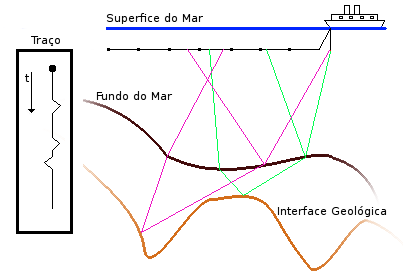
\includegraphics[scale=.7]{navio.png}}
	\caption{Coleta de dados em levantamento sísmico marítimo.}
	\label{fig:sim}
\end{figure}

\subsection{Avaliação e Otimização de Desempenho}

Os resultados apresentados nessa seção foram medidos no sistema \emph{draco} do Grupo de Processamento Paralelo e Distribuído\footnote{\url{http://gppd-hpc.inf.ufrgs.br/}} (GPPD) da Universidade Federal do Rio Grande do Sul (UFRGS). Cada nó da \emph{draco} consiste de 2 processadores Intel Xeon E5-2630 de 8 núcleos, totalizando 16 \textit{threads (Hyper-Threading)}, além de 64 GB DDR4.

Nessa atividade, o objetivo é implementar uma versão paralela e vetorial otimizada da aplicação de Geofísica. O primeiro passo é verificar o desempenho da \textit{cache}, buscando após, encontrar um dos laços para vetorizar. Utilizando o comando: 

\begin{lstlisting}[frame=none, numbers=none]
@\textcolor{mygreen}{\$ perf stat -e cache-misses,cache-references src/6-kernel.exec}@
\end{lstlisting}

verifica-se a taxa de acerto de \textit{cache} da versão original. A taxa retornada nesse caso foi de 27\%, sendo que essa é considerada baixa. Buscando melhorar o desempenho da aplicação, otimizando os acessos a \textit{cache}, utilizou-se a técnica de \textit{loop interchange} para alterar a ordem dos laços. A taxa de acerto para diferentes combinações pode ser vista na Tabela~\ref{tab:oil:cache}. Uma vez que a ordem \texttt{k, Y, X} obteve a maior taxa de acerto, continuou-se com essa, agora buscando efetuar a vetorização.

\begin{table}[!htb]
    \centering
    \caption{Taxa de Acerto da Aplicação Geofísica}
    \label{tab:oil:cache}
    \begin{tabular}{cc}
        \toprule
        Ordem dos laços     & Taxa de Acerto (\%)                 \\ \midrule
        \texttt{X, Y, k}  & 26.9\% \\
        \texttt{Y, k, X}  & 93.6\% \\
        \texttt{k, Y, X}  & 95.8\% \\ \bottomrule
    \end{tabular}
\end{table}

No caso da vetorização, identificou-se que o laço mais interno pode ser vetorizado. Isso é possível, pois a maior parte dos acessos à memória é feita de forma contígua em direção aos pontos em X. O perf também pode ser utilizado para analisar o uso de instruções SIMD via comando: 

\begin{lstlisting}[frame=none, numbers=none]
@\textcolor{mygreen}{\$ perf stat -e simd\_fp\_256.packed\_single,simd\_fp\_256.packed\_double src/6-kernel.exec}@
\end{lstlisting}

verificou-se que após adicionar a diretiva \texttt{omp simd}, o número de instruções \texttt{simd} de precisão simples mudaram de $0$ para $3 429 629 397$. 

Por fim, a Tabela~\ref{tab:results} apresenta os resultados de tempo de execução das diferentes versões utilizando como entrada um cubo de tamanho 512. A versão na qual melhorou-se o desempenho da \textit{cache} foi 5,2$\times$ mais rápida que a versão sequencial. A versão vetorial utilizando unidades vetoriais melhorou o desempenho da aplicação em 3,6$\times$ em relação a versão com \textit{cache} otimizada. A versão paralela em OpenMP foi executada com 32 \textit{threads}, melhorando o desempenho da aplicação em 4,1$\times$. A versão final, que combina todas otimizações, teve o melhor desempenho, de 75,5$\times$ em relação a versão sequencial. Essas e outras propostas de otimização para essa aplicação de geofísica podem ser vistas em diversos trabalhos~\cite{serpa2017strategies, serpa2018optimizing, serpa2018improving, serpa2019optimization}.

\begin{table}[!htb]
\centering
\caption{Desempenho da Aplicação Geofísica}
\label{tab:results}
\begin{tabular}{cc}
\toprule
Versão     & Tempo de Execução (s)   \\ \midrule
Sequencial & 90,6                    \\ 
Cache      & 17,5                    \\ 
Vetorizada &  4,9                    \\ 
OpenMP     &  1,2                    \\ \bottomrule
\end{tabular}
\end{table}